\chapter{portraits des musulmans de France}


Il y a plusieurs études : 
\bi
\item l'Etude Montaigne
\item Etude Européenne de 2017. 76\% des musulmans sont très attachés à leur pays de résidence. A contrario de l'étude de l'IFOP, une confiance plus élevée que le reste de la population en l'Etat et plus exposée aux discriminations.

\ei

\section{L'enquête de l'Institut Montaigne}


\paragraph{La méthodologie de l'Enquête de l'Institut Montaigne}

Ce document présente les principaux résultats d'une enquête réalisée
sur les opinions et les pratiques sociales des personnes musulmanes, et
issues de familles musulmanes, en France. Il s'agit d'une enquête
expérimentale, pionnière en France, dont il convient d'utiliser les
résultats avec précaution et mesure. Elle se distingue par sa volonté
d'interroger la population musulmane dans son ensemble, et non plus
seulement les musulmans parmi la population immigrée.

La question religieuse ne peut être abordée via le recensement général
de l'INSEE, elle ne peut pas l'être non plus par les méthodes de sondage
traditionnelles qui, lorsqu'il s'agit d'interroger des musulmans de
France, ciblent généralement les quartiers où résident un nombre
important d'immigrés. C'est pourquoi nous avons élaboré une
méthodologie, qui vise à extraire d'un vaste échantillon représentatif
de la population résidant en France métropolitaine -- 15 459 personnes
de 15 ans et plus ont été interrogées -- un échantillon spécifique de
personnes musulmanes ou de culture musulmane ; elles représentent 1 029
individus, parmi lesquels 874 se définissent comme « musulmans ». Cette
enquête respecte les principes scientifiques et déontologiques de
l'enquête par sondage. Elle achoppe sur les mêmes difficultés : la marge
d'erreur moyenne d'un sondage effectué auprès d'un échantillon de 1 000
personnes est d'environ 3 \%, celle inhérente à l'analyse d'un
sous-groupe dans ce même échantillon augmente sensiblement et peut
s'élever entre 6 et 8 \%.Les enseignements qu'elle indique reflètent un
état de l'opinion à l'instant de sa réalisation et non pas une
prédiction. Si les calculs sont solides et rigoureux scientifiquement,
les analyses présentées constituent l'une des manières possibles de
traiter les données de cette enquête. Il existe bien évidemment d'autres
méthodes et d'autres choix statistiques, qui pourraient donner lieu à
des résultats différents.

Toutefois, la méthodologie utilisée nous semble constituer le meilleur
compromis afin de produire des résultats fiables. Dans un souci de
transparence, nous publions

\mn{La représentativité de l'échantillon global a été assurée par la
méthode des quotas au regard :


\begin{itemize}
\item
  De critères sociodémographiques (sexe de l'individu, âge de
  l'individu) ;
\item
  De critères socioprofessionnels (profession de l'individu) ;
\item
  De critères géographiques (région administrative, taille d'unité
  urbaine, proportion d'immigrés dans la commune ou du quartier (IRIS)
  de résidence) ;
\item
  De critères civiques (nationalité) ;
\end{itemize}


Ces quotas ont été définis à partir des données du recensement de
l'INSEE pour la population âgée de 15 ans et plus résidant en métropole
(RP-INSEE 2012).}
l'ensemble des procédures techniques employées à chaque étape, ce qui
permet ainsi à n'importe quel autre utilisateur de logiciels
statistiques de pouvoir vérifier et de reproduire nos résultats.
L'analyse d'une enquête si importante ne peut être réalisée au moyen
d'une « boite noire » ; l'usage de techniques vérifiables s'inscrit, au
contraire, en cohérence avec le respect des normes académiques les plus
exigeantes à ce jour.

Cependant, l'analyse complète et approfondie d'une enquête si riche
exige davantage de temps. Les résultats présentés constituent une
première analyse exploratoire, qui devra être précisée et affinée
ultérieurement. Le caractère novateur de cette enquête vise aussi à
identifier les apports et les difficultés méthodologiques liées à
l'étude quantitative des populations religieuses minoritaires dans la
société française ; certaines de ces difficultés nous ont conduits à
faire des choix techniques et pratiques, pour lesquels nous avons
toujours eu à l'esprit la recherche de la précision et de l'exactitude
des résultats.



\subsection{Les caractéristiques socio démographiques des musulmans de France}

La principale tendance sociodémographique de l'islam en France est la
prégnance croissante de la seconde religion du pays auprès des jeunes
générations. Cette dynamique s'explique par la conjugaison de deux
facteurs : la transmission intergénérationnelle d'une part et les
conversions d'autre part.


\begin{itemize}
\item
  
  Le premier apport démographique provient de la transmission
  intergénérationnelle de la religion chez les descendants d'une
  immigration issue de pays musulmans. Cette transmission n'est pas
  toujours linéaire et il s'agit également, parfois, d'un retour au
  religieux des enfants et des petits-enfants issus de familles dans
  lesquelles le religieux était peu important.
  
\item
  
  Le second apport démographique provient des conversions à l'islam
  parmi les personnes n'ayant eu aucun rapport familial avec l'islam au
  cours des générations précédentes.
  
\end{itemize}

\begin{figure}
    \centering
    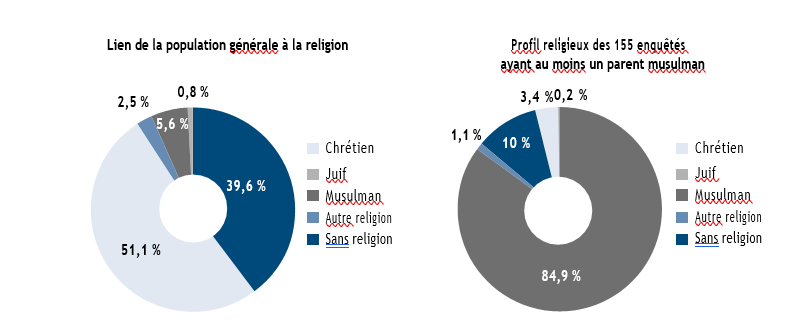
\includegraphics[width=\textwidth]{ImageIslamFrance/profilreligieux.png}
    \caption{Lien de la population générale à la religion Profil religieux
des 155 enquêtés ayant au moins un parent musulman}
    \label{fig:my_label}
\end{figure}

Ces deux dynamiques se combinent et se complètent.

Si 5,6 \% de la population totale des plus de 15 ans7 se déclarent
musulmans dans notre enquête8, cette proportion dépasse les 10 \% chez
les moins de 25 ans.

À l'inverse, deux tendances majeures se dessinent au sein du reste de la
population française :


\begin{itemize}
\item
  
  le déclin persistant de l'affiliation à la chrétienté ;
  
\item
  
  l'accroissement du nombre de personnes qui se déclarent « sans
  religion ».
  
\end{itemize}


Parmi les plus de 75 ans, près de trois répondants sur quatre se
déclarent chrétiens et moins de 20 \% indiquent n'avoir aucune religion,
contre respectivement 30 \% et près de 50 \% chez les moins de 30 ans.


\hypertarget{duxe9mographie}{%
\subparagraph{Démographie}\label{duxe9mographie}}


D'après les résultats de notre enquête, les personnes qui se déclarent
musulmanes représentent 5,6 \% de la population métropolitaine.

Cette proportion est approximative, dans la mesure où la technique du
sondage induit nécessairement des marges d'erreurs qui rendent difficile
l'estimation précise et fiable de ce chiffre ; l'absence de données
officielles, qui permettraient de procéder à un redressement
sociodémographique, contribue également à ce manque de
précision. Cependant, ce résultat est proche d'autres estimations
existantes et apparaît donc pertinent.

Dans l'échantillon initial de 15 459 personnes, plus de 47 \% des plus
de 15 ans se déclarent « chrétiens », 37 \% « sans religion », 6 \% ont
refusé de répondre à cette question et un peu plus de 3 \% s'affilient à
une autre religion minoritaire que l'islam. Ces chiffres rappellent que,
si l'islam est la seconde religion de France métropolitaine, elle est
démographiquement très minoritaire\sn{5 \% des individus interrogés ont refusé de répondre à cette question.}. La structure socioprofessionnelle
de la population qui se définit comme musulmane est marquée par une
surreprésentation des milieux populaires et des populations éloignées de
l'emploi :


\begin{itemize}
\item
  
  plus de 24 \% des musulmans déclarés sont ouvriers ;
  
\item
  
  plus de 22 \% sont employés ;
  
\item
  
  30 \% des musulmans sont inactifs non retraités. Ces personnes ne
  figurent pas dans les statistiques du chômage tel qu'il est calculé en
  France ; elles n'occupent pas d'emploi mais ne sont pas enregistrées
  comme demandeuses d'emploi. Cette catégorie inclut, en revanche, les
  lycéens et étudiants, mais aussi les jeunes à la recherche d'un
  premier emploi10 ;
  
\item
  
  seuls 4,5 \% sont cadres. À titre de comparaison, les cadres
  représentent 10 \% des personnes qui se déclarent « sans religion » et
  plus de 8 \% des chrétiens. \emph{A contrario,} les inactifs non
  retraités ne pèsent que 14 \% et 9,9 \% respectivement dans ces deux
  groupes. Si l'on raisonne en termes de taux d'incidence, les musulmans
  représentent 2,8 \% des cadres mais plus de 10 \% des ouvriers, 7 \%
  des employés et 13,5 \% des inactifs non retraités.
  
\end{itemize}


Cela peut s'expliquer en partie par la pyramide des âges de ce groupe
social, où les jeunes sont significativement plus nombreux. Les
musulmans de l'échantillon sont âgés, en moyenne, de 35,8 ans contre 53
ans pour les chrétiens et 43,5 ans pour les personnes sans religion.

Cet échantillon possède la particularité d'inclure à la fois la
population se déclarant musulmane, et celle qui ne se déclare pas comme
telle mais dont l'un des parents au moins est musulman. Ce dernier
groupe représente 15 \% de la population de l'enquête. Ces personnes
possèdent des ascendants directs musulmans, mais se positionnent
subjectivement comme en dehors de cette religion.






72 \% des répondants se déclarent musulmans lorsque leurs deux parents
sont également musulmans ; 2,7 \% sont musulmans alors que seul leur
père est musulman ; 2,8 \% alors que seule leur mère est musulmane. La
très grande majorité des musulmans, s'inscrit donc dans une transmission
religieuse directe au sein d'une famille dans laquelle les deux parents
sont musulmans.

Cependant, il ne s'agit pas d'un modèle de transmission unique ; ainsi
7,5 \% des personnes se déclarant comme musulmanes déclarent qu'aucun de
leurs parents n'est musulman. Les musulmans sans aucun parent musulman
sont plus nombreux que les musulmans dont seul l'un des deux parents est
musulman. Ce chiffre peut correspondre, de façon schématique, à ce que
l'on considère comme les conversions à l'islam.

Par ailleurs, bien que la religion islamique soit transmise en principe
de façon patrilinéaire, les musulmans dont seul le père est musulman ne
sont pas plus nombreux que ceux dont la seule la mère est musulmane.

Enfin, comme les non-musulmans représentent 15 \% des enquêtés, les
trajectoires de « sortie » de la religion musulmane -- ou de
désaffiliation --apparaissent deux fois plus importantes que les
trajectoires d'entrée ; prenant à rebours les représentations faisant de
l'islam une religion attirant massivement des individus \emph{a priori}
éloignés de cette tradition.

La croissance démographique de l'islam en France suit davantage le
mouvement des générations dans la période post-coloniale que celui d'un
courant idéologique.



\paragraph{Nationalité}

Les données de l'enquête révèlent que 50 \% des enquêtés sont français
de naissance, 24 \% sont français par acquisition et 26 \% sont de
nationalité étrangère. Parmi les Français, nombreux sont les individus
qui possèdent également une autre nationalité, en lien avec leur
trajectoire migratoire ou celle de leurs parents.

La très grande majorité des musulmans étrangers sont originaires du
Maghreb, d'Afrique Subsaharienne ou de Turquie. Les citoyens de ces pays
représentent en effet 23 \% des musulmans de France et représentent plus
de 88 \% des individus ne détenant pas la nationalité française.





\paragraph{Pays d'origine}



\textbf{Pays de naissance du père}
Le père des enquêtés est, dans près de 90 \% des cas, né hors de France.
Ce chiffre semble très élevé, mais il apparaît, dans nos données, plus
faible que dans les résultats de l'enquête \emph{Trajectoire et
Origines} (TeO), conduite par l'INED auprès de la population des
migrants et descendants de migrants de moins de 50 ans en 2008.
Rappelons ici que notre choix méthodologique porte sur l'ensemble de la
population résidant en France, et pas uniquement sur les personnes de
nationalité française. L'Algérie et le Maroc sont les principaux pays
d'origine, avec respectivement 31 \% et 20 \%. La Tunisie représente 8
\% des origines paternelles, les autres pays d'Afrique un peu plus de 15
\% et la Turquie environ 5 \%.


\textbf{Pays de naissance de la mère}
Les mères des enquêtés présentent un profil d'origine nationale
comparable. Il existe cependant des variations significatives : dans
près d'un cas sur cinq (17 \%), les mères sont nées en France, soit 7
points de plus que les pères.

Le croisement des pays de naissance du père et de la mère révèle la
puissance de l'endogamie nationale :


\begin{itemize}
\item
  
  72 \% des enquêtés dont le père est né en France ont aussi une mère
  née en France ;
  
\item
  
  88 \% des personnes ayant un père né en Algérie ont une mère née dans
  le même pays ;
  
\item
  
  91 \% des personnes dont le père est né au Maroc ont une mère née au
  Maroc ;
  
\item
  
  les taux d'endogamie sont comparables pour les personnes originaires
  de Tunisie, de Turquie, ou des autres pays d'Afrique.
  
\end{itemize}

\textbf{Pays de naissance de l'enquêté}
Les 1 029 répondants eux-mêmes sont nés en France dans plus d'un cas sur
deux.

Pour ceux qui sont nés à l'étranger :


\begin{itemize}
\item
  
  14 \% sont nés en Algérie ;
  
\item
  
  près de 13 \% au Maroc ;
  
\item
  
  11 \% principalement en Afrique subsaharienne ;
  
\item
  
  et près de 5 \% en Tunisie.
  
\end{itemize}
\paragraph{Origine sociale}



\begin{figure}
    \centering
    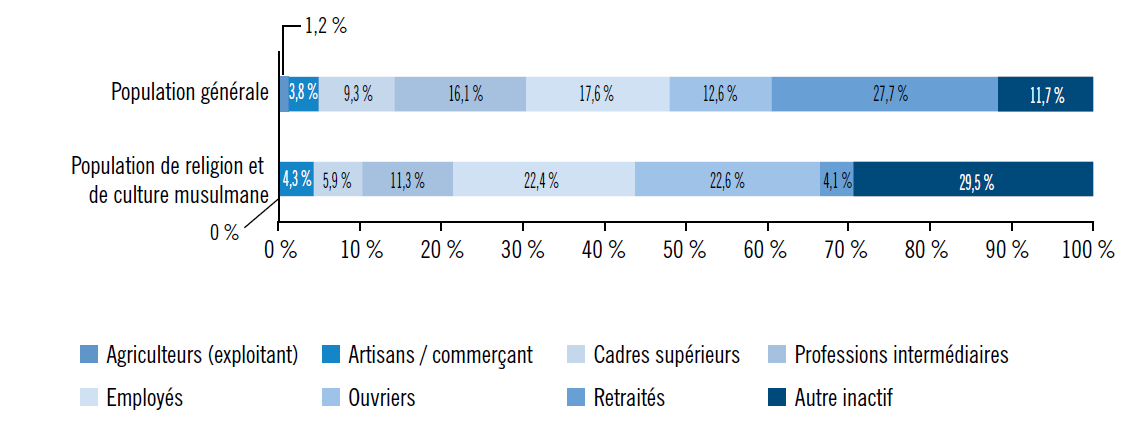
\includegraphics[width=\textwidth]{ImageIslamFrance/OrigineSociale.png}
    \caption{Origine sociale des enquêtés et de la population générale}
    \label{fig:my_label}
\end{figure}

Cette enquête permet également de mesurer la position sociale d'origine
des enquêtés, c'est-à-dire la profession et la catégorie
socioprofessionnelle (PCS) de leur responsable de famille au moment de
l'enquête. Si cette information nous éclaire sur le milieu social
d'origine des enquêtés, en revanche, elle ne nous renseigne pas sur leur
situation individuelle.

De plus, la nomenclature des PCS échoue à saisir la condition sociale
réelle des individus, dans la mesure où parmi la catégorie des personnes
inactives, elle ne distingue ni les étudiants ni les militaires du
contingent ni les « inactifs divers » de moins de 60 ans (non-retraités)
sans activité professionnelle ni les chômeurs n'ayant jamais exercé
d'activité.

On constate une prééminence nette des catégories sociales populaires et
des personnes inactives et une forte sous-représentation des classes
supérieures du salariat (cadres et professions intellectuelles
supérieures).

Les 874 enquêtés qui se déclarent musulmans sont ainsi sous-représentés
parmi les professions intermédiaires (8 \% contre 14,1 \% dans la
population générale) et les cadres et professions intellectuelles
supérieures (4 \% contre 9 \% parmi la population générale) ; et
surreprésentés parmi les ouvriers (24 \% contre 13,1 \%) et les inactifs
(38 \% contre 16,1 \%).




\paragraph{Diplôme}


Alors que leur position sociale d'origine est très modeste, les
musulmans de France se hissent à des niveaux de qualification qui se
rapprochent de la moyenne nationale.

Les personnes titulaires d'un diplôme de niveau BAC + 2 représentent
environ 12 \% de l'échantillon, les titulaires de diplômes plus élevés
20 \% -- dont la moitié possède un titre de niveau BAC +5.
\begin{figure}
    \centering
    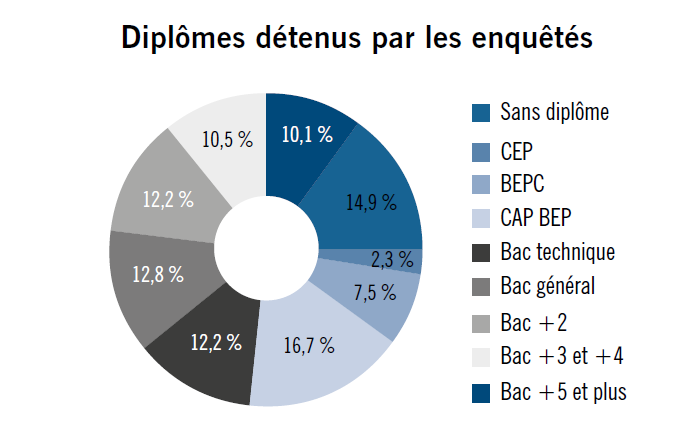
\includegraphics[width=\textwidth]{ImageIslamFrance/Diplome.png}
    \sidecaption{Diplômes détenus par les enquêtés}
    \label{fig:my_label}
\end{figure}



Cependant, une part importante des enquêtés présente également de plus
faibles niveaux de formation :


\begin{itemize}
\item
  
  près de 15 \% ne possèdent aucun diplôme ;
  
\item
  
  environ 25\% ont un niveau inférieur au BAC.
  
\end{itemize}


Cela est le signe d'une polarisation sociale de la population musulmane,
marquée par un accès assez large à l'enseignement supérieur, d'une part,
mais également par la marginalisation scolaire d'une importante
minorité, d'autre part.


Statut dans l'emploi


Si une large part des 1 029 répondants est inactive, la majorité des
personnes actives occupe un emploi stable. Ainsi, plus de 55 \% occupent
un CDI et 10 \% sont fonctionnaires. En revanche, en raison de leur
position sociale plus défavorisée, la précarité touche une part
significative de la population de culture musulmane : plus de 12 \% est
en CDD et plus de 8 \% est en intérim.




\begin{figure}
    \centering
    \includegraphics[width=\textwidth]{ImageIslamFrance/Emploi.png}
    \caption{Statut dans l'emploi des enquêtés}
    \label{fig:my_label}
\end{figure}


\paragraph{Pyramide des âges}


La pyramide des âges témoigne de la jeunesse de la population musulmane
de France. L'âge moyen des répondants est de 35 ans et 75 \% d'entre eux
ont moins de 45 ans.

Ces résultats peuvent être liés à l'évolution démographique de la
population musulmane en France, mais peuvent également être inhérents
aux difficultés que rencontrent fréquemment les instituts de sondage
pour joindre les personnes les plus âgées, notamment parmi les migrants
âgés résidant en France.

Cependant, un nombre important de répondants de plus de 50 ans a pu être
interrogé, complétant en cela l'information sur une population qui ne
figurait pas dans le spectre de l'enquête TeO conduite par l'INSEE et
l'INED.





\subsection{Typologie des musulmans selon leur religiosité}


Nous avons sélectionné plusieurs variables permettant de définir le
rapport au religieux, afin de construire une typologie au moyen d'une
Analyse en Composantes Principales (ACM).

Cette typologie permet de déterminer les dimensions latentes, qui
sous-tendent les rapports au religieux parmi les 1 029 enquêtés. Afin de
rendre ces résultats plus compréhensibles, nous avons ensuite opéré une
classification pour identifier un petit nombre de groupes, parmi les
personnes qui se déclarent musulmanes ou dont les parents sont
musulmans. La construction de l'ACM et de la typologie sont détaillées
en annexe. Là encore, cette typologie n'est que l'une des typologies
possibles. De plus, les critères techniques retenus pour la division des
classes peuvent varier. Aussi, il convient de ne pas attacher trop
d'importance au périmètre et au poids absolu des différentes classes
mais davantage à la structuration générale des opinions et des
attitudes.


\paragraph{Description des classes construites}


Cette typologie permet de distinguer six classes, ordonnées de la
catégorie des individus les plus modérés aux individus les plus
autoritaires :


\begin{itemize}
\item
  La \textbf{première catégorie (18 \% des effectifs) est celle des
  individus les plus éloignés de la religion.} Ils sont favorables à la
  laïcité, ne formulent aucune revendication d'expression religieuse
  dans la vie quotidienne, qu'il s'agisse du monde du travail ou de
  l'école, ne souhaitent pas de nourriture halal à la cantine et sont
  très largement d'accord avec l'idée que la laïcité permet de pratiquer
  librement sa religion. 
\item
  La \textbf{deuxième catégorie (28 \% des effectifs) partage les mêmes
  valeurs.} Les individus qui la composent sont d'accord avec
  l'interdiction de la polygamie et avec l'idée que la loi de la
  République passe avant la loi religieuse. \textbf{Elle se distingue
  par un attachement plus fort à la consommation de nourriture halal et
  une partie de ses membres est favorable à l'expression religieuse au
  travail.}
\item
  La \textbf{troisième catégorie (13 \% des effectifs) est plus
  ambivalente.} Elle s'oppose au niqab et à la polygamie, mais elle
  conteste l'idée selon laquelle la laïcité permet de pratiquer
  librement sa religion. Sans être radicale, elle critique le modèle
  républicain, \emph{a minima} dans ses modalités d'application.
  \textbf{Une forte minorité de ces membres souhaite d'ailleurs pouvoir
  exprimer sa religion sur son lieu de travail.}
\item
  La \textbf{quatrième catégorie (12 \% des effectifs) se distingue de
  la troisième par une plus grande acceptation de la laïcité. En
  revanche, elle critique massivement l'interdiction de la polygamie en
  France} tout en condamnant absolument le niqab, rejeté par 95 \% des
  membres de ce groupe. Cette catégorie réunit beaucoup de musulmans
  étrangers résidant en France.
\item
  La \textbf{cinquième catégorie (13 \% des effectifs) représente les
  individus qui présentent des traits autoritaires :} 40 \% de ses
  membres sont favorables au port du niqab, à la polygamie, contestent
  la laïcité et considèrent que la loi religieuse passe avant la loi de
  la République. Dans leur immense majorité, les membres de ce groupe ne
  considèrent pas que la foi appartienne à la sphère privée, ils sont
  d'ailleurs majoritairement favorables à l'expression de la religion au
  travail.
\item
  La \textbf{sixième catégorie (15 \% des effectifs) se distingue de la
  cinquième en prônant une vision plus « dure » des pratiques
  religieuses.} En revanche, elle valorise la foi comme un élément privé
  et non comme un élément public. Presque tous ses membres valorisent le
  port du niqab et près de 50 \% contestent la laïcité tout en étant
  favorables à l'expression de la religion sur le lieu de travail.
\end{itemize}


Ces six catégories racontent trois histoires différentes :


\begin{itemize}
\item
  \textbf{Groupe 1 (catégories 1 et 2 représentant 46 \% des musulmans
  de France) sont soit totalement sécularisés soit en train d'achever
  leur intégration dans le système de valeurs de la France
  contemporaine, qu'ils contribuent d'ailleurs à faire évoluer par leurs
  spécificités religieuses.} Ils ne renient pas pour autant leur
  religion, souvent identifiée au halal, et ont une pratique religieuse
  nettement plus régulière que la moyenne nationale ;
\item
  \textbf{Groupe 2 (catégories 3 et 4) : il est plus composite et
  s'inscrit clairement dans une position intermédiaire. Fiers d'être
  musulmans,} les individus qui le composent revendiquent la possibilité
  d'exprimer leur appartenance religieuse. Très pieux (la charia a une
  grande importante pour eux, sans passer devant la loi de la
  République), ils sont souvent favorables à l'expression de la religion
  au travail, et ont très largement adopté la norme halal comme
  définition de « l'être musulman ». Ils rejettent très clairement le
  niqab et la polygamie et acceptent la laïcité ;
\item
  \textbf{Groupe 3 (catégories 5 et 6) : Autoritaire au point de vue religieux. il est le plus problématique.
  Il réunit des musulmans qui ont adopté un système de valeurs
  clairement opposé aux valeurs de la République.} Majoritairement
  \textit{jeunes}, peu qualifiés et peu insérés dans l'emploi, ils vivent dans
  les quartiers populaires périphériques des grandes agglomérations. Ils
  se définissent davantage par l'usage qu'ils font de l'islam pour
  signifier leur révolte que par leur conservatisme. Si certains
  considèrent
que la laïcité leur permet de vivre librement leur religion  ou
considèrent que la foi est une affaire privée\sn{12 « Diriez-vous que la foi religieuse est pour vous d'abord quelque
chose de privé ? »}, on peut davantage y
lire une attitude de retrait et de séparation vis-à-vis du reste de la
société que la compréhension de ce que signifie la laïcité. \textbf{28
\% des musulmans de France} peuvent être regroupés dans ce groupe qui
mélange à la fois des attitudes autoritaires et d'autres que l'on
pourrait qualifier de « sécessionnistes ». \textbf{L'islam est un moyen
pour eux de s'affirmer en marge de la société française.}
\end{itemize}

\begin{Synthesis}
Sur la nourriture Halal comme marqueur, \CB souligne que des études qualitatives minorent cette importance.
\end{Synthesis}

À partir de ces éléments, il est possible d'étudier les caractéristiques
sociodémographiques des groupes identifiés selon la typologie du rapport
à la religion que nous venons d'établir.


\paragraph{Description sociodémographique des groupes}


\textbf{Effet de l'âge}

L'effet de l'âge est l'un des mécanismes les plus puissants en matière
d'analyse du rapport au religieux. \textbf{Le groupe 1, le plus éloigné
de la religion, est très peu représenté parmi les jeunes générations.}
S'il représente toujours près de la moitié des individus chez les plus
de 40 ans, il ne concerne plus qu'un tiers des répondants les plus
jeunes.

Ce mouvement est compensé par la croissance du groupe 3, \textbf{le plus
rigoriste religieusement et le plus autoritaire, qui passe d'environ 20
\% de la population des plus de 40 ans à près de 50 \% chez les cohortes
les plus jeunes.}

En revanche, le poids du groupe intermédiaire (groupe 2) est à la fois
faible et stable quelles que soient les cohortes étudiées.






Il n'est pas ici possible de vérifier statistiquement qu'il existe un
effet d'âge et non un effet de génération, mais ce scénario apparaît
comme le plus plausible. \textbf{Le mouvement à l'œuvre semble se
caractériser par une intensification de l'identité religieuse des
nouvelles cohortes (par rapport à leurs aînés au même âge).} L'hypothèse
alternative invite à considérer qu'au cours de leur vie les personnes de
culture musulmane vivant en France s'éloignent des formes les plus
rigoristes de rapport au religieux. Si cette hypothèse ne peut pas
\emph{a priori} être rejetée ici, elle paraît peu probable au regard des
autres travaux publiés sur ces questions.


Effet de la catégorie socio-professionnelle


L'effet de la catégorie socio-professionnelle sur le rapport au
religieux est, là aussi, significatif.

\textbf{Les personnes qui appartiennent aux catégories sociales les plus
favorisées (Cadres, Professions intermédiaires) sont nettement
surreprésentées dans le groupe 1, et sous représentées dans le groupe 3}
-- le plus autoritaire. En revanche, le lien identitaire fort à l'islam
est surreprésenté dans les milieux populaires, chez les ouvriers et les
employés, et plus fortement encore parmi les inactifs, qui regroupent
notamment les jeunes n'ayant jamais occupé d'emploi et les étudiants.

Les logiques d'âge et de classe sociale se combinent et permettent
d'identifier le renforcement probable des attitudes religieuses
autoritaires parmi les jeunes et dans les catégories populaires de la
population musulmane résidant en France. \textbf{Ce mouvement n'est pas
spécifique aux jeunes musulmans des milieux populaires. Il s'observe
également chez les jeunes qui se définissent comme chrétiens ou sans
religion, mais s'exprime par d'autres opinions et comportements que
l'affiliation identitaire à l'islam.}

\begin{figure}
    \sidecaption{Catégorie socio-professionnelle des enquêtés}
    \centering
    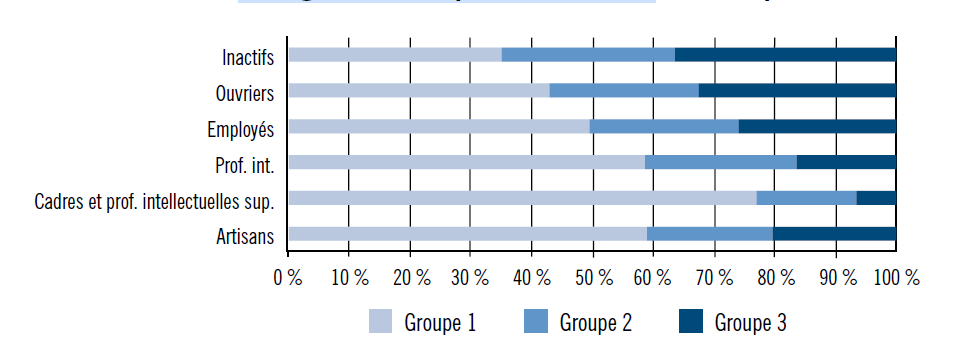
\includegraphics[width=\textwidth]{ImageIslamFrance/CSP.png}

    \label{fig:my_label}
\end{figure}




\textbf{Effet du type d'activité
} L'analyse des effets du statut d'activité confirme cela. \textbf{Les
personnes les mieux insérées sont celles qui ont le plus de chance de
rejeter les attitudes les plus rigoristes dans le rapport à l'islam.}
Cela ne signifie en rien que la religion soit moins importante pour eux,
ou qu'ils soient « moins musulmans » que les autres. Les variations du
rapport au religieux, telles qu'identifiées dans cette typologie, sont
des différences de nature et non des différences de degré.


\begin{figure}
    \sidecaption{Activité exercée par les enquêtés des 3 groupes 
    Les chefs d'entreprises, les fonctionnaires et les salariés en CDI se
situent en dehors du groupe 3 dans plus de 80 \% des cas. En revanche,
\textbf{les personnes en position plus précaire (stagiaires, salariés en
intérim ou en CDD) sont celles qui, parmi les actifs, sont le plus
susceptibles d'appartenir aux groupes qui présentent les attitudes les
plus intransigeantes.}}
    \centering
  
  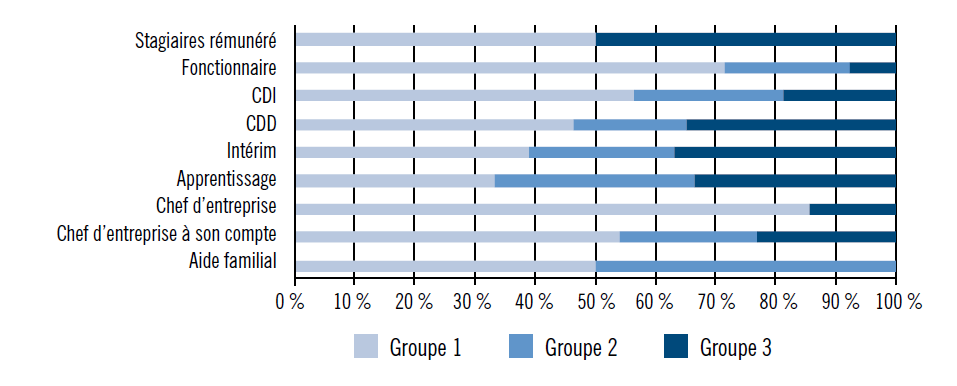
\includegraphics[width=\textwidth]{ImageIslamFrance/activite.png}
    \label{fig:my_label}
\end{figure}






\textbf{Effet du genre}
La comparaison entre les hommes et les femmes sur le rapport au
religieux indique que les femmes apparaissent légèrement surreprésentées
dans le groupe 3, mais ces écarts sont minimes une fois rapportés aux
dynamiques sociales et générationnelles. 

\textbf{Effet du type de lien à l'islam}

Nous avons cherché à déterminer si ces dynamiques sont présentes chez
les seules personnes qui se déclarent musulmanes, ou si elles se
retrouvent également parmi les personnes dont l'un des deux parents est
musulman mais qui ne disent pas elles-mêmes musulmanes.



\begin{figure}
    \sidecaption{Répartition des enquêtés dans les 3 groupes Les résultats peuvent paraître surprenants : \textbf{si les
non-musulmans présentent un rapport plus distancié au religieux que les
musulmans, l'écart est relativement mince.} C'est notamment le cas pour
le groupe 3, celui qui rassemble les plus autoritaires : près de 20 \%
des enquêtés qui se déclarent non-musulmans soutiennent les mêmes
positions.}
    \centering
  
  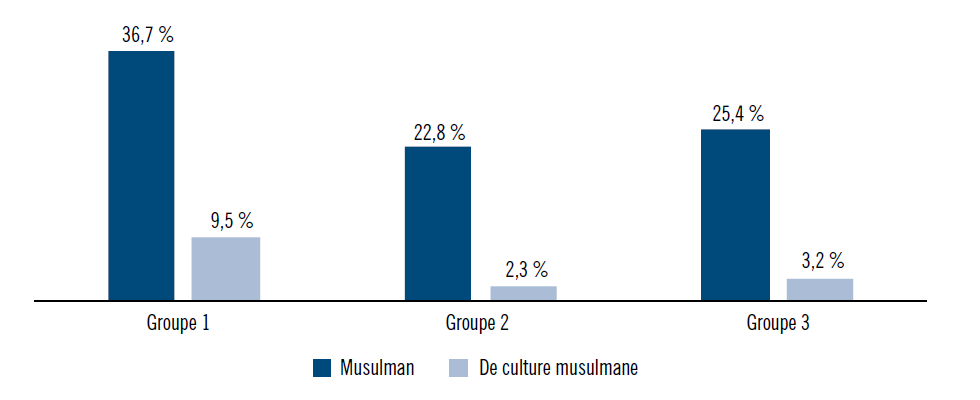
\includegraphics[width=\textwidth]{ImageIslamFrance/lienIslam.png}
  
\end{figure}



\begin{Synthesis}
Cette situation montre que l'islam est souvent davantage le support
d'une attitude de rébellion qu'une adhésion spirituelle qui entraînerait
une pratique particulièrement rigoriste.
\end{Synthesis}


Pour affiner ce résultat, il est important de comparer les groupes selon
le rapport familial à l'islam (un parent, deux parents ou aucun parent
musulman). Les différences sont faibles et fragiles statistiquement,
cependant \textbf{il semble que ce soit les personnes converties
(musulmanes sans parent musulman) qui présentent les attitudes les plus
autoritaires.}

Il faut cependant nuancer ces éléments car ces profils sont minoritaires
en nombre dans tous les groupes sociaux.


  \subsection{Quelle pratique de l'Islam ?}


\paragraph{Halal, un pilier de l'islam} La consommation de viande halal fait l'objet d'un intérêt important pour
les musulmans, qui l'identifient de plus en plus au simple fait d'être
musulman : être musulman, c'est être halal (par opposition à « haram »).
De fait, \textbf{de nombreuses représentations erronées circulent.
Ainsi, plus de 40 \% des répondants musulmans souscrivent à
l'affirmation selon laquelle la consommation de viande halal
constituerait l'un des 5 piliers de l'islam,} ce qui est évidemment
faux.

70 \% des répondants déclarent « toujours » acheter de la viande halal,
22 \% en achètent « parfois » et seulement 6 \% « jamais ».

Comme l'ont montré plusieurs travaux depuis l'enquête \emph{Banlieue de
la République \sn{\cite{Kepel:Banlieue}}}, la consommation de nourriture halal devient un
marqueur d'appartenance au groupe social des musulmans, y compris chez
les individus n'étant pas -- ou peu --
religieux. On décèle ici les signes d'un rapport au religieux qui se vit
d'abord par les normes et les pratiques sociales, et de façon secondaire
par les pratiques rituelles ou cultuelles.

Cette consommation halal est forte dans l'ensemble de la population
musulmane et
« d'origine » musulmane. Ainsi, huit répondants sur dix souscrivent à
l'affirmation selon laquelle les enfants devraient avoir la possibilité
de manger halal à l'école. Ce chiffre est moindre, mais reste très
élevé, chez les répondants de culture musulmane ne se déclarant plus
musulmans (67 \%).

Ce marqueur social semble s'être autonomisé de la référence religieuse :
la consommation halal est devenue normale -- au sens propre du terme. La
norme sociale dépend alors moins de la foi et de la théologie que d'un
mode de vie partagé.

 il n'y a pas d'effet d'âge net sur
la consommation de nourriture halal parmi la population interrogée.
Ainsi, plus de 80 \%, toutes les classes d'âges confondues, déclarent
acheter « toujours » ou
« parfois » du halal. Et c'est logiquement que 80 \% des musulmans
interrogés souscrivent à l'affirmation suivante : \emph{« Les enfants
devraient pouvoir manger halal dans les cantines scolaires ».}

De façon analogue, le niveau de qualification ne semble pas avoir
d'influence nette sur la consommation de halal. La répartition est là
encore relativement homogène parmi l'ensemble des répondants.



En ce qui concerne la question plus spécifique des repas halal proposés
dans les cantines scolaires, les résultats présentent également une
relative homogénéité parmi l'ensemble des 1 029 personnes interrogées.
On observe néanmoins que 35 \% des répondants titulaires d'un diplôme de
niveau bac+5 ou plus disent ne pas être d'accord avec la proposition «
les enfants devraient pouvoir manger halal dans les cantines scolaires
», alors que moins d'une personne sur cinq partage cette opinion parmi
le reste des enquêtés.


\textbf{Ainsi, une majorité de musulmans consomme régulièrement du
halal. L'attachement à cette pratique n'est ni révélateur d'un rapport
plus radical à la religion ni un indicateur de fondamentalisme
religieux.}



\paragraph{Le port du voile : quelles motivations
?}


Le port du voile est une question ancienne dans le rapport à l'islam en
France. C'est par la question du port du voile dans les établissements
scolaires que l'Union des Organisations islamiques de France (UOIF) est
apparue sur la scène médiatique et a touché une audience importante dans
les années 1990 et au début des années 2000. Plus récemment, de nombreux
débats ont eu lieu autour de l'interdiction du port du voile intégral
(loi de 2009), sur la possibilité d'une extension aux Universités de
l'interdiction du voile à l'école, adoptée en 2004, ou encore sur les
conditions de l'interdiction du port du voile dans les entreprises
(notamment avec l'affaire Baby Loup\sn{La crèche Baby Loup est un établissement associatif privé ouvert à Chanteloup-les-Vignes en 1991, qui est surtout connu pour avoir été le théâtre d'affrontements judiciaires à la suite du licenciement, en 2008, d'une salariée de la crèche au motif qu'elle portait un foulard islamique, alors que le règlement intérieur de l'association imposait le respect des principes de laïcité et de neutralité à son personnel.}).


\textbf{Environ 60 \% des 1 029 enquêtés considèrent que les jeunes
filles devraient pouvoir porter le voile au collège et au lycée.} En
revanche, cette position n'est soutenue que par 37 \% des personnes de
culture musulmane -- dont les parents sont musulmans mais qui ne se
déclarent pas musulmanes. Ainsi, la question du voile reste nettement
plus clivante, y compris parmi les musulmans, que ne l'est celle de la
consommation de viande halal.

\textbf{Environ 65 \% des musulmans -- de religion ou de culture -- se
déclarent favorables au port du voile}, \sn{« \textit{Personnellement, êtes-vous favorable à ce qu'une femme porte le
voile -- le hijab ? }» « \textit{Personnellement, êtes-vous favorable à ce qu'une femme porte le
voile intégral -- niqab ou burqa ?} » }
Dans les deux cas,
environ 10 \% des répondants adoptent une position de retrait individuel
en choisissant la réponse \emph{« c'est son choix, chacun fait ce qu'il
veut ».}
et 24 \% sont
favorables au principe du port du voile intégral
Contrairement à l'opinion dominante qui voudrait que les hommes soient
plus conservateurs que les femmes, le port du voile est rejeté par 26 \%
des hommes mais seulement par 18 \% des femmes. Les hommes sont
également plus enclins à déclarer que \emph{« chacun fait ce qu'il veut
».} \textbf{Ces résultats témoignent d'une adhésion idéologique d'une
part importante de la population féminine musulmane au port du voile,
allant jusqu'à l'acceptation du voile intégral (pour 28 \% des femmes).}

Cependant, l'approbation du port du voile ne signifie en rien que les
comportements des individus correspondent à la norme ainsi revendiquée,
sachant que le port du voile intégral est interdit dans l'espace public.
Peut-être peut-on lire dans ces résultats très élevés une forme de
provocation, suite notamment aux nombreux débats sur le port des signes
religieux musulmans dans l'espace public.

La pratique sociale la plus répandue reste le non-port du voile \sn{Question posée : \textit{Vous-même, portez-vous le voile (qu'il s'agisse du
hijab ou du niqab)} ? Réponses possibles : Oui : oui, sauf sur le lieu de
travail ou d'étude -- Oui, mais rarement ; Non : non, mais vous l'avez
porté autrefois ; non, et vous ne l'avez jamais porté}.
\textbf{Ainsi, les deux tiers des femmes de culture musulmane déclarent
ne pas porter le voile.} 57 \% déclarent ne l'avoir jamais porté et 8 \%
déclarent l'avoir déjà porté, mais ne plus le faire aujourd'hui.

Environ 35 \% des répondantes déclarent porter le voile (tout le temps
ou de manière épisodique). Si ce chiffre semble en augmentation au
regard des enquêtes réalisées en 2003 sur ces questions (+ 11 points),
il reste très éloigné des 65 \% évoqués précédemment :

\begin{Synthesis}
Il y a une vraie différence entre le porte du voile, minoritaire et son acceptation, très large chez les musulmans pratiquants, y compris chez les femmes. Seulement 12\% des femmes le portent de façon intermittente.
\end{Synthesis}

\begin{itemize}
\item
  
  23 \% des femmes déclarent « toujours » porter le voile ;
  
\item
  
  7 \% déclarent le porter sauf sur le lieu de travail ou d'étude ;
  
\item
  
  5 \% déclarent le porter « rarement ».
  
\end{itemize}


Ces chiffres indiquent que les pratiques de port intermittent sont
relativement peu fréquentes et que les femmes qui mettent et retirent le
hijab selon les contextes (scolaires, professionnels) sont assez peu
nombreuses au regard de l'ensemble de la population de culture
musulmane.

Ces résultats sont précieux, car ils s'inscrivent dans une dynamique
générationnelle inverse. Là encore, les effectifs sont faibles et les
résultats demandent à être consolidés. Cependant, il apparaît que les
femmes de 25 à 50 ans déclarent plus fréquemment porter le voile (40 \%)
que les 15-25 ans (environ 10 points de moins). \textbf{Il est probable
que l'interdiction du port du voile au collège et au lycée ait une
influence sur le relativement faible port du voile chez les jeunes, y
compris hors des établissements scolaires.}


Cette dynamique générationnelle qui imprime sa marque sur les pratiques,
n'influe pas sur les opinions. Ainsi, les répondants de 15 à 25 ans sont
majoritairement favorables à l'autorisation de porter le voile dans
l'enseignement secondaire.


En comparant les réponses de femmes musulmanes portant le voile et
celles des femmes musulmanes ne portant pas le voile, on constate que
leurs motivations et leurs perceptions sont distinctes. Les musulmanes
portant le voile motivent cette pratique par l'obligation religieuse (76
\%), par des enjeux de sécurité (35 \%), par la volonté de montrer leur
appartenance à la foi musulmane (23 \%), mais seules 6 \% déclarent le
faire par contrainte ou par imitation des autres.

Les femmes musulmanes ne portant pas le voile jettent un regard plus
critique sur cette pratique. Elles sont 66 \% à considérer que les
femmes portant le voile le font par obligation religieuse, 44 \% par
volonté de montrer qu'elles sont musulmanes (+ 20 points), 27 \% par
mimétisme (+ 21 points), 24 \% par contrainte (+ 18 points).

\begin{Synthesis}
Une vraie différence sur la vision du voile selon qu'on le porte ou non. 
{Seul point de convergence net : le port du voile pour des
raisons de sécurité est là aussi cité par 35 \% des répondantes.}
\end{Synthesis}

\paragraph{Quelles autorités religieuses
?}


\textbf{Les résultats de notre enquête mettent en évidence le déficit de
notoriété et de légitimité des organisations islamiques en France.} Le
rapport au religieux évolue rapidement dans les plus jeunes générations.
Il se traduit par une défiance accrue vis à vis des institutions, y
compris des institutions musulmanes.

Ainsi, plus des deux tiers des répondants déclarent ne pas connaître le
Conseil Français du Culte Musulman (CFCM). Parmi les 300 répondants
connaissant l'institution, seuls 28 \% déclarent se sentir représentés
par cette structure. \textbf{Ce ne sont \emph{in fine} que 9 \% des
personnes se définissant comme musulmanes en France qui déclarent se
sentir représentées par le CFCM}\textbf{.}

En complément, nous avons interrogé les enquêtés sur leur proximité avec
d'autres institutions et d'autres figures de l'islam en France\sn{En tant que musulman, vous sentez-vous représenté par le CFCM
(Conseil Français du Culte Musulman) ? Oui -- Non
-- Refus de répondre
« En tant que musulman, vous sentez-vous proche... ? »
\begin{itemize}
\item
  « D'intellectuels comme Tariq Ramadan »
\item
  « De religieux comme Tareq Oubrou ou Dalil Boubakeur »
\item
  « De l'U.O.I.F. (Union des Organisations Islamiques de France) »
\end{itemize}
Et pour chacune des propositions : -- Oui -- Non -- Ne connaît pas -- Refuse de répondre -- Ne sait pas
}. 
L'UOIF
(Union des Organisations Islamiques de France), qui n'est plus
représentée au CFCM après avoir boycotté les élections de 2013, est
éclipsée. Alors qu'elle organise chaque année au Bourget l'un des
principaux événements musulmans d'Europe, plus de 30 \% des personnes
musulmanes déclarent ne pas la connaître et seuls 12 \% s'en disent
proches. Il est cependant probable que les mouvements et structures liés
à l'UOIF bénéficient d'une visibilité et d'une reconnaissance plus
grande.

Les personnalités religieuses comme Tareq Oubrou (Recteur de la mosquée
de Bordeaux) ou Dalil Boubakeur (Recteur de la grande mosquée de Paris)
ne recueillent pas davantage de soutien, étant inconnues de près de 30
\% des musulmans, seuls 16 \% se sentent « proches » de ces deux
personnalités.

Tariq Ramadan \label{Theol:TRamadan1}, en revanche, bénéficie d'un soutien plus large. 37 \% des
enquêtés musulmans s'en déclarent proches, alors que seuls 15 \%
déclarent ne pas le connaître. Cette déconnexion entre rapport aux
organisations et aux responsables religieux témoigne de la recherche
d'une représentation sociale des musulmansqui passe davantage par des personnalités publiques, dont les moyens
d'actions sont plus proches de ceux de la sphère politique (meetings,
réunion publiques, conférences, émissions de télévision, etc.).



\paragraph{Quelle fréquentation des mosquées
?}


La fréquentation des mosquées est une question importante. La
représentation sociale des musulmans repose aujourd'hui sur le CFCM,
dont la composition dépend en partie de l'importance des différents
lieux de culte. Par ailleurs, les mosquées sont une interface,
présentées dans le débat public à la fois comme des lieux de diffusion
des idéologies radicales et des lieux d'enseignement du religieux et de
la langue arabe. Elles occupent donc une place importante dans
l'ensemble des dynamiques étudiées.

Selon les données de notre enquête, environ \textbf{30 \% des 1 029
répondants musulmans ne se rendent jamais à la mosquée}\textbf{.} De
plus, 30 \% supplémentaires ne s'y rendent que pour les grandes
célébrations du ramadan ou moins souvent. \textbf{Ce sont donc près de
60 \% des musulmans qui ont un rapport distancié ou inexistant avec les
lieux de culte}\textbf{.}

Environ 15 \% des musulmans se rendent à la mosquée une fois par
semaine, généralement pour la prière du vendredi. Les pratiquants les
plus assidus représentent environ 12 \% de la population musulmane. Ces
derniers se rendent plusieurs fois par semaine dans les lieux de culte,
et 5 \% des individus déclarent s'y rendre quotidiennement. \sn{« À quelle fréquence allez-vous à une mosquée ou une salle de prière
? »
\begin{itemize}
\item
  Au moins une fois par semaine • Chaque jour • Plusieurs fois par
  semaine • Une fois par semaine • Au moins une fois par mois •
  Seulement à l'occasion des fêtes religieuses • Moins souvent • Jamais
  • Refuse de répondre • Ne sait pas.
\end{itemize}
La fréquentation des salles de prière est considérée, dans notre
enquête, comme équivalente à la fréquentation des mosquées.
}

Si le lien aux lieux et institutions cultuels apparaît relativement
distendu, cela ne signifie pas que la religiosité est absente de la vie
d'une majorité de musulmans.

Au contraire, la pratique de la prière, y compris l'usage des cinq
prières quotidiennes est répandue, même chez les individus ne
fréquentant pas ou peu les mosquées\sn{ « Et faites-vous la prière ? »
\begin{itemize}
\item
  Oui, 5 fois par jour • Oui, occasionnellement • Oui, mais seulement
  pour le Ramadan et les Aids • Non, jamais
\item
  Refuse de répondre • Ne sait pas.
\end{itemize}}.

Si plus de neuf individus sur dix qui se rendent chaque jour à la
mosquée respectent les cinq prières quotidiennes, c'est également le cas
de 50 \% des musulmans ne se rendant dans les lieux de culte que pendant
le ramadan, et de 45 \% de ceux s'y rendant moins souvent. On constate
donc, là encore, le \textbf{développement d'une religiosité importante
mais relativement indépendante des institutions, des lieux de culte et
des structures musulmanes, tout en aspirant à une piété forte et à la
reconnaissance de pratiques religieuses ayant trait à l'organisation de
la vie collective au quotidien.}




  \subsection{Leur rapport à la France, à ses institutions et à la société}
  
  
    \paragraph{Attachement}



Analysons désormais le rapport à la France et à ses institutions de la
population de culture musulmane. Nous avons demandé aux enquêtés s'ils
considéraient \emph{« possible »} qu'une personne de culture musulmane soit élue
président de la République dans les années à venir. Les opinions sont
très partagées, 45 \% des enquêtés sont enclins à penser que cela est
possible, 45 \% considèrent le contraire. Ces résultats témoignent d'une
relative confiance dans la capacité de la société française à évoluer.
Ces dynamiques peuvent également être nourries par l'exemple américain,
près de huit ans après la victoire de Barack Obama lors de l'élection
présidentielle de 2008.

Nous avons cherché à savoir ce que les personnes qui se déclarent
musulmanes
  ou les personnes de culture musulmane -- considèrent comme « important
  » et
« non important ».

\textbf{Ces résultats révèlent la très forte aspiration d'une immense
majorité de la population musulmane d'accéder à un meilleur statut
social.} Plus de 90 \% des répondants considèrent important d'avoir un
emploi stable, plus de 85 \% valorisent le fait d'avoir « de bons
diplômes » et plus de 65 \% tiennent pour important le fait de devenir
propriétaire de leur logement.

Les pratiques traditionnelles, telles que la valorisation du fait
d'avoir un garçon plutôt qu'une fille sont reléguées (65 \% des
répondants considèrent que cela n'est pas important). La volonté d'aller
vivre dans un pays musulman constitue un engagement plus fort et indique
davantage d'ambivalence : plus de 30 \% des enquêtés considèrent cela
comme important. C'est principalement le cas lorsque la perspective de
l'amélioration de leur condition sociale paraît s'éloigner en France,
sous l'effet des discriminations et des inégalités, parfois perçues
comme la conséquence d'un « complot » contre les musulmans\sn{ « En France, les musulmans sont victimes d'un complot »}. Ces 30 \%
sont également
à mettre en relation avec le fait que plus de 25 \% des enquêtés ne sont
pas de nationalité française.

\paragraph{Défiance}


\textbf{Les impôts et les inégalités sociales sont très largement
dénoncés, faisant de la question sociale la priorité des musulmans
interrogés, bien avant les questions religieuses ou identitaires.}
Cependant, l'idée selon laquelle \emph{« En France les musulmans sont
victimes d'un complot »} recueille un assentiment important, avec près
de 37 \% de réponses positives et 8 \% de non-réponse. Ces perceptions
alimentent la défiance d'une partie des musulmans de France, qu'ils
soient de nationalité française ou non.

La défiance s'exprime moins directement envers le pays qu'à travers la
condition des musulmans en France, dénoncée comme le fruit d'une
infériorisation injuste, historiquement héritée et doublée d'un mépris
pour l'islam ; dont la défense passe, pour certains -- notamment chez
les jeunes de milieux populaires --, par une dynamique de réaffirmation
de leur identité religieuse.

En quoi ces dynamiques influencent-elles le rapport à l'autre et les
interactions avec les autres groupes sociaux ?


\subparagraph{Ouverture à l'autre et
mixité}


Afin d'étudier les interactions des enquêtés avec le reste du corps
social, nous avons listé une série de comportements en leur demandant
s'ils se reconnaissaient ou non dans ces pratiques\sn{Vous-même, est-ce que vous\ldots{} ? Acceptez de vous faire soigner par médecin {[}femme{]} / {[}homme{]} ou un/une infirmier/ère {[}femme{]} / {[}homme{]} Écoutez de la musique Serrez la main à une {[}femme{]} / {[}homme{]} Faites la bise à une {[}femme{]} / {[}homme{]} Acceptez d'aller dans une piscine mixte (où il y a à la fois des hommes et des femmes)}.

Les résultats indiquent que la grande majorité des personnes musulmanes
acceptent de se faire soigner par un médecin du sexe opposé (92,5 \%),
près de 88 \% serrent la main d'une personne de sexe opposé et 89 \%
écoutent de la musique ; ce qui ne signifie pas que les 10 \% restant
soient opposés à la liberté d'écouter de la musique.

Cependant, certains items reçoivent un niveau de réponse négative plus
élevé : 30 \% des répondants ne font pas la bise à une personne du sexe
opposé et 33 \% refusent de se rendre dans une piscine mixte. Là encore,
ce sont les rapports entre hommes et femmes qui font apparaître une
déconnexion entre les pratiques d'une minorité non négligeable de la
population musulmane et les usages communs de la population majoritaire
en France.

\paragraph{Opinions politiques sur la société
française}


Comment l'ensemble des résultats précédents se traduisent-ils
politiquement ? Pour le savoir, nous avons soumis aux enquêtés de
religion et de culture musulmane des questions sur leur positionnement
subjectif ; en leur demandant où ils se situaient sur un axe
gauche-droite allant de 0 à 10 -- 0 étant le plus à gauche et 10 le plus
à droite.


\begin{figure}
    \centering
        \sidecaption{Positionnement Gauche / Droite}
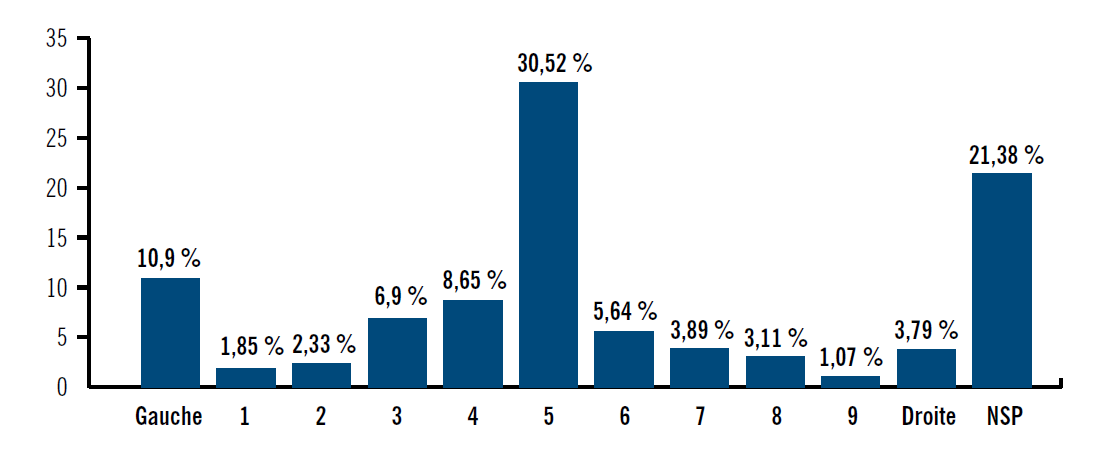
\includegraphics[width=\textwidth]{ImageIslamFrance/GaucheDroite.png}

  
\end{figure}


28 « Habituellement, on classe les individus politiquement sur une
échelle qui va de la gauche à la droite. Personnellement, où vous
classeriez-vous sur cette échelle ? 0 signifie qu'en termes de
positionnement politique vous êtes à très à gauche, 10 signifie que vous
êtes très à droite, et les notes intermédiaires permettent de nuancer
votre jugement. »

Les réponses sont claires : si la gauche capte un soutien légèrement
plus important que la droite, notamment suite à une mobilisation massive
en faveur de François Hollande lors de l'élection présidentielle de
2012, plus de 50 \% des répondants refusent de se prononcer ou se
positionnent au « centre », c'est-à-dire ni à droite ni à gauche et non
pas comme des sympathisants de courants centristes.

\begin{figure}
    \centering
    \sidecaption{Positionnement politique gauche/droite selon le rapport à l'islam}
    
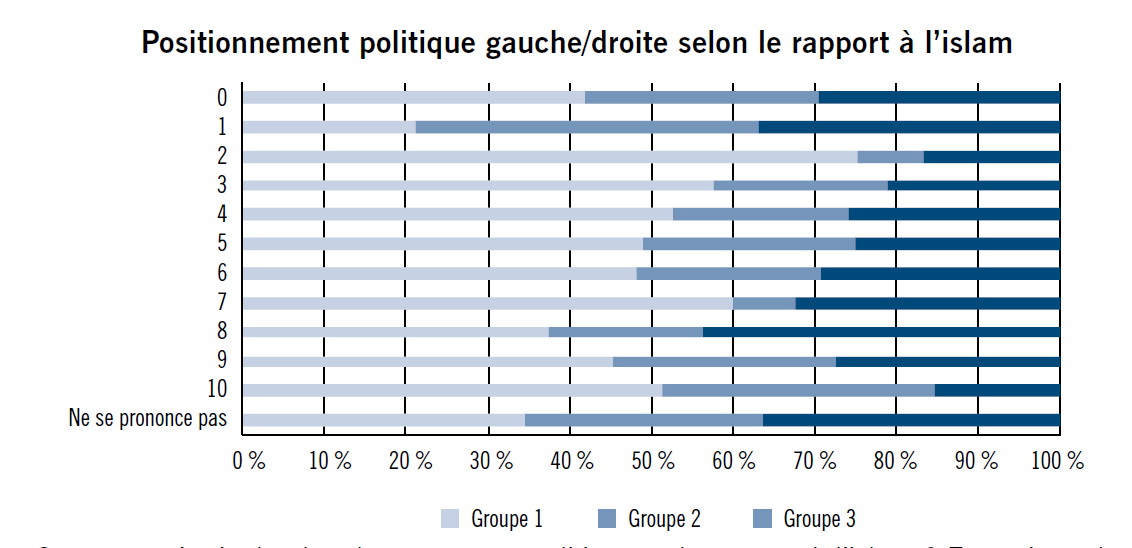
\includegraphics[width=\textwidth]{ImageIslamFrance/GaucheDroitepargroupe.png}
 
\end{figure}



Comment s'articule alors le rapport au politique et le rapport à l'islam
? En croisant la nomenclature en 6 groupes issus de la typologie avec
l'échelle des positionnements gauche-droite, on constate que \textbf{les
musulmans les plus libéraux et les plus éloignés du religieux sont ceux
qui s'identifient le plus fortement à la gauche. Les groupes les plus
autoritaires ont davantage une propension à se placer hors du spectre
politique gauche-droite ou à se rapprocher de la droite.}


\paragraph{Le rapport au politique}


Le rapport au politique ne passe pas seulement par les opinions. Il est
également façonné par les pratiques et les comportements. La pratique
politique la plus fréquente reste, en démocratie, l'exercice du vote.
Toutefois, pour voter en France, il faut nécessairement être de
nationalité française et être inscrit sur les listes électorales. Nous
avons filtré les réponses des 1 029 enquêtés afin de ne conserver que
celles des personnes qui se déclarent françaises et sont âgées de plus
de 18 ans. Elles constituent la « base électorale théorique » parmi
laquelle des électeurs inscrits peuvent être recrutés.



Au sein de cette population, près d'un quart des répondants ne sont pas
inscrits sur les listes électorales. Ce chiffre, très important, a un
impact en aval sur toute la chaîne de la participation et de la
représentation politique. Par ailleurs, parmi la population musulmane en
France, un quart des individus ne disposent pas du droit de vote car ils
ne sont pas français, et parmi les 75 \% restant, un quart
supplémentaire d'entre eux ne sont pas inscrits sur les listes
électorales.

L'effet de l'abstention contribue à affaiblir encore le niveau de
mobilisation, accroissant l'écart entre le poids social et le poids
politique de la population de religion ou de culture musulmane qui
s'avère fortement sous représentée dans les urnes.

Nous avons tenté de reconstituer le comportement électoral des musulmans
lors de l'élection présidentielle de 2012 : 27 \% des enquêtés alors
inscrits sur les listes électorales s'étaient abstenus et 10 \%
déclarent avoir choisi le vote blanc ou nul\sn{30 Avez-vous voté au premier tour de l'élection présidentielle en avril
2012 ? \begin{itemize}
\item
  Vous avez voté pour un des candidats en présence
\item
  Vous avez voté blanc ou nul
\item
  Abstention
\item
  Vous n'étiez pas inscrit sur les listes électorales
\item
  Refuse de répondre
\end{itemize}}.
Ainsi, par effet de
composition, \textbf{seuls 33 \% des personnes de religion ou de culture
musulmane ont voté pour l'un des deux candidats du second tour de 2012
;} alors que ce scrutin est celui au cours duquel la participation des
quartiers populaires a été la plus forte dans l'histoire politique
récente de la France.



\paragraph{Conclusions de l'enquête}


Si l'analyse de cette enquête mérite une exploitation plus exhaustive,
elle apporte, d'ores et déjà, des réponses inédites -- construites de la
façon la plus rigoureuse possible --, sur les comportements sociaux et
politiques des personnes musulmanes et de culture musulmane vivant en
France. Sans assignation \emph{a priori} et dépassant les seuls critères
d'âge ou de nationalité, elle cherche à s'approcher au plus près d'une
réalité sociale encore mal connue, pour laquelle les études
quantitatives visant à produire des résultats représentatifs font
particulièrement défaut. Nous sommes évidemment prudents sur les
résultats quantitatifs obtenus : il est très compliqué de mesurer des
croyances, les biais sont nombreux et cette enquête étant inédite, nous
ne disposons pas d'éléments de comparaison qui pourraient permettre de comparer et de redresser les
réponses recueillies. L'enquête permet donc d'identifier des tendances
et il est difficile d'interpréter davantage ces résultats.

Ce portrait des musulmans de France décrit une réalité très contrastée.
La première, à rebours de beaucoup d'idées reçues, est qu'il n'y a ni «
communauté musulmane », ni « communautarisme musulman » unique et organisé. Il existe des Français
de culture et de confession musulmane, dont le sentiment d'appartenance
à la communauté musulmane est, d'abord et avant tout, individuel : peu
d'engagement associatif au nom de l'islam, des choix politiques aux
élections très faiblement influencés par « l'islamité » réelle ou
supposée d'un candidat, la faiblesse du sentiment de destinée
collective, très peu d'écoles confessionnelles.

Certains traits de comportements se dessinent nettement et peuvent
néanmoins les distinguer du reste de la communauté nationale : ils
apparaissent très nettement plus conservateurs que la population
générale en ce qui concerne les relations entre les hommes et les femmes
(virginité avant le mariage, obéissance attendue de la femme envers son
mari). Ces différences varient très faiblement selon le genre des
personnes interrogées.
\begin{Synthesis}
Trois marqueurs communs les rassemblent : (i) la norme alimentaire
halal, devenue une façon d'être-au-monde islamique, (ii) une pratique
religieuse très nettement supérieure au reste de la société et (iii) un
soutien au port du voile, qui reste majoritaire malgré de forts clivages
internes.
\end{Synthesis}

Porteurs d'une vision de la société différente sur certains sujets,
soucieux d'affirmer certaines spécificités, ils pourraient s'organiser
pour peser sur le débat public. Rien de tout cela n'émerge : ils votent
très peu, s'affichent majoritairement au centre (alors qu'ils votent
traditionnellement à gauche), n'ont jamais créé de partis communautaires
ou religieux et continuent à garder un certain espoir envers la capacité
d'intégration de l'ordre politique national ; la moitié d'entre eux
croit possible l'élection d'un président musulman dans les prochaines
années et leurs problèmes essentiels sont économiques et sociaux bien
avant d'être religieux ou identitaires.

Mais leur portrait ne se limite pas à ces traits communs. Ce sont
d'ailleurs les différences et les divergences qui dominent l'analyse. Un
large groupe, qui regroupe

50 \% d'entre eux, suit un chemin qui va les mener progressivement vers
la sécularisation ; ce qui ne signifie pas qu'ils vont abandonner la
norme alimentaire halal ou que leur pratique religieuse va brutalement se réduire. Leur
système de valeurs leur permettra de s'insérer dans une société
française qu'ils contribuent à faire évoluer par leurs spécificités
religieuses.

Les 25 \% médians, qui présentent les caractéristiques du conservatisme
religieux, sont l'enjeu de la bataille politique et idéologique qui a
débuté. Cette bataille est à l'œuvre dans le dernier groupe, le plus
problématique, qui regroupe environ 25 \% des musulmans de France avec,
parmi eux, beaucoup de jeunes, peu qualifiés et peu insérés dans
l'emploi qui vivent dans les quartiers populaires périphériques des
grandes agglomérations à forte densité d'immigrés. Ce groupe ne se
définit plus par son conservatisme, mais par l'utilisation qu'il fait de
l'islam afin de mener une véritable rébellion idéologique vis-à-vis du
reste de la société française, tant ses valeurs et ses comportements
sont opposés à la norme et aux habitus communs.

Essayons de comprendre les raisons de cette situation. On entre ici sur
un terrain fait de complexités, d'influences multiples,
d'incompréhensions réelles et de questionnements identitaires avec des
causes à la fois endogènes et exogènes à la société française.

La crise de transition du monde arabe, qui abandonne très rapidement son
système d'organisation traditionnel et se trouve confronté à une
modernité à inventer, a évidemment un impact sur les Français musulmans
; tout comme la succession de crises politiques et géopolitiques qui
affectent cette partie du monde. La transformation des sociétés arabes,
d'une part, la violence des conflits -- et les interventions
occidentales -- habitent leur quotidien et créent des sentiments duaux
: ils savent que l'organisation traditionnelle n'est plus un recours
face à leurs difficultés quotidiennes, que la sécurité qu'aurait pu
représenter le lien avec des sociétés traditionnelles stables a disparu.
Ils se représentent également leurs pays d'origine, et leur culture,
comme pris en otage par le jeu des puissances occidentales (Palestine,
Irak, Syrie, etc.) et s'identifient aux victimes du Moyen-Orient. Un
être au monde victimaire se construit peu à peu, avec ses ennemis : les
Américains, les Israéliens, les Occidentaux, qui ont tôt fait de se
transformer dans la bouche de certains radicaux en « Croisés » ou en «
Juifs ». L'antisémitisme est ainsi devenu un marqueur d'appartenance
pour ce groupe\sn{31 Dominique Reynié, \emph{L'antisémitisme dans l'opinion publique
française,} Nouveaux éclairages, Fondapol, novembre 2014}, qui se pose à la fois en victime de puissances
hostiles et en porteur d'une solution : l'islam. Un islam qui apparaît
comme une réponse au malaise identitaire car il permet de répondre à la
question


\begin{quote}
  « Qui suis-je si je ne suis ni vraiment français ni citoyen du pays
d'origine de mes parents ? »  
\end{quote}
Un islam qui se veut en rupture avec celui
des grands-parents, des parents qui ont baissé la tête, des parents qui
ont été les victimes de ceux qu'ils dénoncent par ailleurs (l'Occident,
la colonisation voire les « Croisés »). Un islam qui de fait n'est plus
transmis par la famille mais par des groupes politico-religieux divers
(Tariq Ramadan, Frères musulmans, Tabligh, salafistes, voire État
islamique), qui jouent sur le sentiment de victimisation et sur la
nécessité de « relever la tête », quitte à faire peur ; ce qui permet
également de dépasser la condition de victimes.

Mais, les causes extérieures sont loin d'expliquer à elles seules ce
phénomène : les difficultés de l'intégration jouent un rôle majeur.
Passer d'un système de valeurs patriarcales, fondé sur la solidarité
entre les frères, où le statut de la femme -- et notamment de la fille
-- est inférieur à celui de l'homme -- et notamment du garçon --, au
modèle républicain qui valorise les filles à l'école (les filles
d'immigrés y réussissent bien mieux que les garçons et échouent aussi
bien moins que les garçons d'origine immigrée), c'est une révolution
copernicienne dans les familles, maghrébines notamment.

Ce choc anthropologique se produit au moment même où la société
française connaît quatre crises de transformation, qui affectent au
premier chef les enfants d'immigrés musulmans. La désindustrialisation,
d'abord, qui frappe de plein fouet les ouvriers. Les immigrés venus
d'Afrique du Nord, de Turquie et moins significativement d'Afrique
sub-saharienne ont été recrutés afin de reconstruire la France de
l'après-guerre, de participer à l'essor industriel des Trente Glorieuses
et de répondre à une demande de main-d'œuvre peu qualifiée que le
\emph{« grand déversement des campagnes vers les villes »,} cher à
Alfred Sauvy, ne suffisait pas à satisfaire. Quand, à la fin des années
1970, la sidérurgie d'abord, les charbonnages et l'automobile ensuite,
puis toute l'industrie française a commencé à réduire ses effectifs de
production sur le territoire national, les familles d'immigrés ont payé
un tribut très lourd en matière de chômage et de précarité économique et
sociale.

Dans le même temps, les structures d'encadrement politique des milieux
populaires ont peu à peu disparu : le parti communiste a initié son
déclin, les syndicats n'ont jamais su inclure véritablement les immigrés
et leurs enfants, le gaullisme n'est jamais parvenu à les toucher (à
l'exception des harkis). L'Église est, par définition, restée un monde
étranger à leur vie quotidienne et spirituelle. L'école, victime des
effets ghetto, n'a pas pu leur offrir les moyens de l'ascension sociale.
Quant à l'État il n'a pas pu, ou pas su, leur donner les cadres
idéologiques et matériels qui auraient pu leur permettre de s'élever
au-dessus de leur condition de départ. Restait donc l'islam.



La montée de l'islamisme et du fondamentalisme ne sont donc pas des
phénomènes exogènes à la société française. Les idéologues islamistes
ont mis en place un dispositif intellectuel et idéologique pour
s'immiscer dans une société au moment où cette dernière le leur
permettait. Leur montée en puissance est, d'une certaine manière,
\textbf{la conséquence} de l'éclatement de l'idée nationale
traditionnelle, et non sa cause comme beaucoup voudraient le croire : ce
serait rassurant en effet, on en connaîtrait les coupables -- en
l'occurrence les islamistes -- et on pourrait les balayer d'un revers de
main.

Ce grand mouvement s'inscrit, enfin, dans le contexte général d'une
société française bloquée par une lutte de pouvoir entre les
générations, où l'insertion des jeunes sur le marché du travail, sur le
marché du logement, sur le marché des idées, est devenue pour tous
extrêmement difficile, y compris pour les diplômés de l'enseignement
supérieur qui pour nombre d'entre eux quittent la France. Ceux qui
restent subissent le fléau des stages à répétition et des emplois
précaires. Dans ce contexte, la situation des enfants d'immigrés est
extrêmement difficile, car s'ajoutent à ces difficultés des
discriminations particulièrement élevées que l'on mesure aujourd'hui
précisément\sn{Institut Montaigne, \emph{Discriminations religieuses à l'embauche :
une réalité,} octobre 2015.}. Le résultat est ce que l'Ined et l'Insee appelle un
\emph{« déni de francité »}, ressenti par 40 \% des enfants d'immigrés.

Ignorer ces causes endogènes à la société française serait commettre une
très grave erreur. La montée du fondamentalisme religieux est notre
échec à tous, ce n'est pas seulement « leur problème à eux ». Ne pas
entendre ce qu'il dit du sort réservé à la jeunesse française, du
fonctionnement de la société, de ses blocages, serait passer à côté
d'une réalité trop évidente pour ne pas déranger. Croire, enfin, que
l'on va résoudre le problème par la seule dénonciation de la
manifestation des signes d'appartenances religieux, c'est méconnaître
l'ampleur de la révolte qui gronde tout en la renforçant : ces signes
sont des marqueurs identitaires. Plus on attaque des marqueurs
identitaires, plus on renforce évidemment l'expression de cette
identité.

Les solutions sont doubles. Elles concernent d'abord la France, dans son
ensemble : pour les réinsérer dans le projet collectif national, il faut
s'interroger sur les moyens de redonner de l'espoir aux classes
populaires. Améliorer le fonctionnement de l'école, redonner de la
compétitivité à certains territoires périphériques, choisir des
politiques sociales qui luttent contre les avantages acquis des «
insiders », mesurer les effets du reflux de la dépense publique sur des
publics et des territoires en difficulté\ldots. La liste est longue,
elle dit les échecs de plusieurs décennies de politiques publiques
françaises.

Au-delà de ces éléments conjoncturels, l'enjeu est de les inclure à
nouveau dans le récit national, en tant que musulmans, mais aussi et
surtout en tant que Français. Le pire serait que l'on réponde à la
pulsion de révolte d'une partie des jeunes, fondée sur l'idée qu'il y a
« eux » -- les « impurs » -- et « nous » -- les musulmans fiers de
l'être, mais victimes de l'islamophobie ambiante -- par un discours
politique fondé lui aussi sur cette dichotomie. À cette différence que
le « eux » serait « les jeunes musulmans dangereux » et le « nous » les
« bons » Français menacés. Dans le contexte sécuritaire actuel, cette
tentation sera difficile à éviter. Mais, il faut savoir résister aux
provocations et à la haine. Surtout quand elles proviennent d'une part
significative de la jeunesse française. La France peut faire la guerre à
Daech, elle ne peut pas entrer en guerre avec une partie de sa jeunesse.

Pour éviter de tomber dans le piège tendu par les extrémistes, le
discours politique doit s'appuyer sur les exemples de réussite des
Français de culture et de confession musulmane et sur la majorité
silencieuse, insérée avec succès dans la société française. Il convient
d'envoyer deux types de messages : l'un au grand public, à qui il faut
rappeler encore et toujours que l'on peut être Français et musulman sans
que cela ne pose le moindre problème, l'autre aux jeunes tentés par le
fondamentalisme religieux, en réaffirmant qu'il n'y a pas de plafond de
verre infranchissable.

La deuxième piste de solutions concerne l'islam qu'il faut construire et
qui sera français en tant qu'il sera porteur d'une représentation du
monde soluble avec les valeurs nationales, qu'il luttera contre
l'hégémonie idéologique des porteurs de l'islam politique, qu'il
produira et qu'il diffusera de la connaissance religieuse, qu'il sera
financé par de l'argent français et qu'il s'appuiera, enfin, pour
réaliser ce plan d'action, sur des femmes et des hommes nouveaux, issus
de la majorité silencieuse des musulmans de France.

L'islam en France est fragmenté et divers : il n'existe non pas un islam
mais des islams, nourris et diffusés par des institutions et des
mouvements nationaux, des organisations transnationales ou des États
étrangers. Cette multiplicité d'acteurs dans le champ musulman français,
les tensions qu'ils suscitent au niveau local et populaire, les
rivalités qu'ils nourrissent, contribuent à la complexité de la
compréhension de l'islam en France et à l'opacité de la situation. Aussi
est-il opportun de passer en revue ces différents acteurs de l'islam en
France, au niveau national et institutionnel comme au niveau local et
populaire. Ce tableau montre que ces acteurs et ces différents niveaux
n'agissent pas en silo mais nourrissent au contraire de véritables
interactions.


%-------------------------------------------------------------------------------

\section{L'enquête ARTE 2020}


\mn{Nous, Français musulmans}


Est ce que les musulmans sont tiraillés entre islam et Français ? que pensent les français musulmans ?
\paragraph{Sondage IPSOS} \mn{Du 18 juillet au 3 août 2017 \href{https://www.ipsos.com/sites/default/files/ct/news/documents/2020-01/lislam_et_la_societe_francaise.pdf}{Résultat du sondage}}
On peut vivre son rapport à l'islam en dehors des carcans traditionnels. Depuis les marches 2015, l'incompréhension des français devant les français musulmans est patente. 
2015 était très compliqué pour les français musulmans. 
59\% des musulmans disent avoir été questionnés par des non-musulmans au sujet des attentats mais 2/3 disent comprendre ces questions. Les Français ont donc échangé, discuté. 
Ghaleib Bencheikh, \emph{Président de la fondation de l'Islam de France} :
\begin{quote}
    Quatre I caractérisant le mot Islam en France : Identité, Insurrection, Islam, Insécurité.
\end{quote}
Avec une question sur les media. les rares voix qui essayent de mettre un peu d'ordre ne sont pas entendues et pas assez de relais médiatiques. 
Eva Janadin, \mn{ cofondatrice de « VOIX DʼUN ISLAM ÉCLAIRÉ »}, parle d'une islamisation de l'Islam. mais il y a le fantasme du grand remplacement.
Hassame Bentabet \mn{Sociologue, spécialiste de l'Islam}, ce qui est visible est une minorité, mais active.  Les français ont incarné l'image d'un musulman figé, uni.  
Les français se déclarant musulmans :
\bi
\item 6\% se déclarent athées
\item 38,5\% se déclarent non-pratiquants
\item 55,5\% croyants pratiquants
\ei

\begin{quote}
    donne du sens face à un monde consumériste 
    faire du bien autour de moi
    
\end{quote}

Karim El Karoui : une dichotomie très forte entre une vision rigoriste et identitaire et une vision intégrée.


\paragraph{les musulmans pratiquants}
\bi
\item 7,5\% pratiquants très occasionnels
\item 12\% pratiquants réguliers
\item 26\% pratiquants rigoristes intégrés, ce sont eux que l'on voit le plus. Application rigoriste. Ce retour au religieux se trouve aussi dans le monde juif et chrétiens. Mais les tendances les plus fortes au sein de l'islam sont les plus radicales.
\item 10\% pratiquant radicalisés isolés
\ei

Marcel Gauchet pose la question de l'intégration de la société. Renvoyé à la religion par rapport à un malaise identitaire.

\paragraph{Marche des beurs} En 1983, la marche pour l'égalité et contre le racisme, la marche des beurs, nous avions enfin l'espoir d'une citoyenneté de plein droit. On ne parle pas du religieux. \emph{Cahier de doléance} : le modèle est le tiers etat de la révolution française. Le slogan "touche pas à mon pote" fut un camouflet avec la main de fatima et de mettre sous la responsabilité des autres et non pas de l'état.
Peu à peu, évolution vers l'étiquette de musulman. 

44\% des musulmans pensent que les français ne les respectent pas.
Les hommes sont fortement discriminés (blind test) et pas les femmes.

\paragraph{par rapport au rejet, renforcement de l'identité musulman}. 72\% des musulmans se disent favorables au port du voile. Une vraie coupure par rapport aux anciens musulmans, qui considèrent seulement à 18\% qu'ils souhaitent le voile.

\paragraph{le foulard de Creil en 1989} question de l'identité française très profonde. Le foulard a été aussi une question pour les jeunes musulmanes pour s'affirmer face à leurs parents ou la société.
Gauchet : 
\begin{quote}
    un signe est fait pour être interprété et c'est pour cela que les signes se prêtent extraordinairement au conflit.
    SOit une sujetion des femmes soit un signe de liberté. Un point de dogme se discute mais pas un signe. 
\end{quote}
La question du voile est assez hystérique même si que 10\% des femmes musulmanes le portent. Symboliquement, la femme voilée est un acte de régression féminisme, un signe communautarisme, islamisation. On n'en sortira pas avec de telle vue. Cela devrait être un choix individuel.
Pourtant 47\% des musulmans disent qu'ils ressentent une pression d'autres musulmans, en particulier ceux qui vivent dans un quartier musulman, une cité. je suis rejetée dans les quartiers. 
Mais alors ce n'est plus le même voile, si c'est obligatoire. 

\paragraph{le voile questionne la place de la femme}. Celui qui suit l'Islam ne peut voir la nudité, mais avec Burqini, on \emph{bricole le religieux}. 78\% des musulmans pensent que les hommes et les femmes ont le même rôle dans la société. 
D'un point de vue théologique, une vraie égalité. Mais la construction humaine, les jurisconsultes ont cristalisé une place de la femme subalterne. 
Marcel Gauchet : 
\begin{quote}
    le monde religieux a toujours été un monde de sujetion pour les femmes.
\end{quote}
Pour l'islam, c'est un monde rural transposé en France. \mn{Comores : les femmes héritent de tout.}

\paragraph{Musulman sécularisé} : 38\% musulmans non pratiquant. une rationalisation du croire, 

\paragraph{Les apostats} De l'ordre du coming out. 6\% des musulmans se disent athées.  Naim Aka Lamine (humoriste). Comment garder son lien avec sa famille. Le sujet de l'apostat est souvent une ligne rouge. "moi, je vais à la Mosquée pour ne pas montrer que j'ai quitté l'islam". 


\begin{Synthesis}
Pas de stéréotype du Français musulman, depuis l'athée au rigoriste. Question homme femme, acceptation de l'alterité (celui qui n'a pas la même culture ou religion que moi), homosexualité. 
\end{Synthesis}


\subsection{Rupture de 2015 : l'islam devient une question publique}

Beaucoup de musulmans étaient à la manif du 11 janvier 2015. 
Qu'est ce qu'attendent les musulmans ?
\bi
\item ne pas être stigmatisé. Eviter l'injonction de désolidariser avec le terrorisme. "je n'ai rien à voir avec les fous".
\item 88\% des français musulmans jugent intolérable de rejoindre Daesh (12\% comprennent Daesh ?).
\ei
\paragraph{Je ne suis pas charlie} un symbole de défiance : le mouvement \emph{je ne suis pas Charlie} sur les réseaux sociaux. La réponse de L'imam à une de ses élèves pour la minute de Charlie par rapport à des enfants en Palestine. 
\begin{quote}
"est ce que vous accepteriez que vos voisins fassent la fête si une personne mourrait chez vous. C'est juste que le Charlie, c'est un drame chez nous et on doit être solidaire".

\end{quote}

\paragraph{Pratiquants radicalisés Isolés} D'après le sondage, il serait 10\% de pratiquants radicalisés isolés (et 26\% de pratiquants rigoristes intégrés). 
On caricature le choix dans les quartiers populaires soit de la petite délinquance soit du salafisme. L'Arabie Saoudite a exporté le salafisme. 7 bn \$ par an. Dans internet, on va voir "Check Google". 
Le conservatisme donne des excuses à la radicalisation. Quand il y a justification à la violence. 
\paragraph{Ghettoisation} En cours dans les quartiers; avec tolérance à la violence : 4 fois plus forte dans ces zones que dans les autres zones.

La décennie 90 : c'est là que tout bascule. Avec les premiers combats en Tchéchénie. En 1992, en Yougoslavie, le salafisme apparait en Europe. David Vallat, djihadiste. Le 25 juillety 1995, le djihadisme apparait à Paris avec l'attentat de la station Saint Michel. 
Khaled Kelkal, intelligent, scolarisé en France, bon élève au Lycée. Petite délinquance et en prison, se radicalise. 5\% des français musulmans ont une bonne image de Daesh, 10\% pour les jeunes de moins de 35 ans et moins que le SMIC. Il suffit que passe du sens, une mauvaise réponse à une vraie question, le déclassement. On leur propose un monde "wonderland islamique". L'islamique s'occupe de "ton lien à Dieu", imposer sa vision du monde aux autres. Convaincre les musulmans qu'ils sont le vrai islam.

\paragraph{Image de l'Islam } Une partie de l'image négative des musulmans vient des pays musulmans (Pakistan, Arabie Saoudite), qui ne sont guère des modèles. 7,5\% des musulmans estiment que leurs valeurs ou croyances sont mal acceptées par la société française. Cela dit, ce doit être la même chose pour les cathos.

\subsection{Représenter les musulmans}
\paragraph{Un travail littéraire} relire les textes, interpréter le texte

\paragraph{Conseil Français du Culte Musulman} Penser la théologie en France.  Seul 24\% des musulmans connaissent précisément les prescriptions du CFCM.
Poids des pays d'origine; poids étatique. La proximité est telle avec l'Algérie et le Maroc qu'on a accepté leur intervention. Aujourd'hui, c'est utilisé pour contrôler les diasporas.
300 imams sont des fonctionnaires étrangers (turcs ou marocains) sur 2800.
Après 2000, la plupart des musulmans ne parlent pas arabes ni ne connaît pas la réalité française : 
\begin{Ex}
\begin{quote}
je demande à un imam marocain ou d'Arabie Saoudite ce que je dois faire avec le voile et que si je n'enlève pas le voile, je perds mon travail : tu n'as pas besoin de travailler sans se rendre compte que le travail est non seulement un moyen financier mais d'estime de soi.
\end{quote}
\end{Ex}

\paragraph{La France est une puissance musulmane} Plus de musulman que le Qatar. 

\paragraph{Altérité}

69\% des musulmans prêts à épouser un non musulman.
Laicité : liberté de conscience et liberté de culte. 
Marcel Gaucher : 
\begin{quote}
    tout le monde occidental est Laic comme en France mais comme cela a été obtenu de façon conflictuelle, la France se sent obligés de le dire à haute voix. 
\end{quote}
81\% des musulmans de France considèrent que la laïcité est positive en France. Les minorités convaincus sont toujours plus fortes que les majorités molles. 
\mn{Mohamed Majrafil, Imam positif sur la France. }

\paragraph{Armée et Fierté d'être français}
20 000 militaires musulmans en France, 10 fois plus que ceux qui vont chez Daech. Une base intéressante car aspect politique car Français. Même chiffre que la population française pour la fierté française (82\%).
\emph{Le faire ensemble}, mieux que vivre ensemble.

